%% ITEM 0 TYPE Section
\section{Introduction}%% ITEM 1 TYPE Frame
%% ITEM 1 TYPE Frame
\begin{frame}
\begin{center}
\LARGE\textbf{Introduction: Vector Embeddings and ANNS}
\end{center}

\vspace{0.5cm}

\begin{itemize}
    \item \textbf{Vector embeddings} convert words/concepts into numerical vectors
    \item Enable AI systems to understand semantic relationships
    \item Example: $\heartsuit \overset{\text{embedding}}{\implies} [0.124, 1.564, ...]$
    \item Similarity measured by \textbf{distance metrics}:
    $$dist(x, y) = \sqrt{\sum_{i=1}^{n}(x_i - y_i)^2}$$
    \item Smaller distance = higher similarity \cite{wang2024distance}
\end{itemize}
\end{frame}%% ITEM 2 TYPE Frame
%% ITEM 2 TYPE Frame
\begin{frame}
\begin{center}
\LARGE\textbf{The ANNS Problem}
\end{center}

\vspace{0.5cm}

\begin{itemize}
    \item \textbf{Core problem}: Find vectors most similar to query vector
    \item \textbf{Nearest Neighbor Search (NNS)}: Exact solution (computationally expensive)
    \item \textbf{Approximate Nearest Neighbor Search (ANNS)}: Efficient approximate solution
    \item Applications: Information retrieval, pattern recognition, RAG \cite{arora2018hd}
    \item \textbf{Graph-based approaches} offer high quality and low latency
\end{itemize}
\end{frame}%% ITEM 3 TYPE Frame
%% ITEM 3 TYPE Frame
\begin{frame}
\begin{center}
\LARGE\textbf{Vector Embeddings and ANNS}
\end{center}

\vspace{0.5cm}

\begin{itemize}
    \item \textbf{Vector embeddings}: Convert words/concepts to numerical vectors
    \item Enable AI to understand semantic relationships
    \item Similarity measured by distance metrics (e.g., Euclidean)
    \item \textbf{ANNS problem}: Find vectors most similar to query
    \item \textbf{Approximate solution}: Efficient search with relaxed accuracy
    \item Applications: Information retrieval, pattern recognition, RAG
\end{itemize}
\end{frame}%% ITEM 4 TYPE Section
%% ITEM 4 TYPE Section
\section[Methods - Partitioning \& Search Algorithms]{Methods - Partitioning \& Search Algorithms}%% ITEM 5 TYPE Section
%% ITEM 5 TYPE Section
\section[Methods: CSPG - Partitioning \& Search Algorithms]{Methods: CSPG - Partitioning \& Search Algorithms}%% ITEM 6 TYPE Frame
%% ITEM 6 TYPE Frame
\begin{frame}
{CSPG: Core Idea \& Partitioning Strategy}
\vspace{-5mm}
\begin{columns}
\begin{column}{0.5\textwidth}
\begin{itemize}
\item \textbf{Goal}: Improve graph-based ANNS with optimal speed-accuracy tradeoff
\item \textbf{Key insight}: Use partitioning to create sparser, smaller proximity graphs
\item \textbf{Partitioning}: Randomly divide dataset $\mathcal{D}$ into groups
\item \textbf{Routing vectors}: Shared vectors across groups enable cross-partition search
\item \textbf{Benefit}: Sparse graphs allow larger steps for fast initial approach
\end{itemize}
\end{column}
\begin{column}{0.5\textwidth}
\begin{figure}
\centering
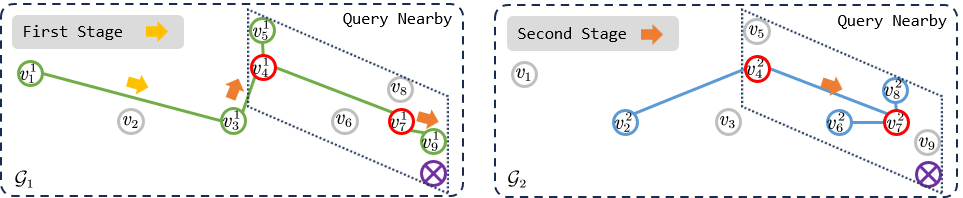
\includegraphics[width=0.95\textwidth,height=0.7\textheight,keepaspectratio]{picture/method.png}
\caption{CSPG partitioning with routing vectors (red)}
\end{figure}
\end{column}
\end{columns}
\end{frame}%% ITEM 7 TYPE Frame
%% ITEM 7 TYPE Frame
\begin{frame}
{Two-Stage Search Algorithm}
\vspace{-5mm}
\begin{columns}
\begin{column}{0.5\textwidth}
\begin{itemize}
\item \textbf{Stage 1: Fast Approaching}
\begin{itemize}
\item Greedy beam search on single partition
\item Small candidate set size $ef_1$
\item Quickly zones into query's nearby region
\item Minimal expansions for speed
\end{itemize}
\item \textbf{Stage 2: Precise Search}
\begin{itemize}
\item Cross-partition dynamic expansion
\item Larger candidate set size $ef_2$
\item Expands routing vectors across all partitions
\item Maximizes search space for accuracy
\end{itemize}
\end{itemize}
\end{column}
\begin{column}{0.5\textwidth}
\begin{figure}
\centering
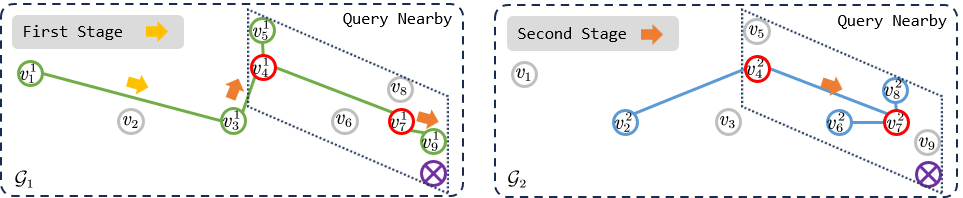
\includegraphics[width=0.95\textwidth,height=0.7\textheight,keepaspectratio]{picture/method.png}
\caption{Stage 1 (yellow) \& Stage 2 (orange)}
\end{figure}
\end{column}
\end{columns}
\end{frame}%% ITEM 8 TYPE Frame
%% ITEM 8 TYPE Frame
\begin{frame}
{CSPG: Key Advantages}
\centering
\vspace{5mm}
\begin{itemize}
\item \textbf{Speed}: Sparse graphs enable fast initial approach with larger steps
\item \textbf{Accuracy}: Cross-partition expansion maximizes search space
\item \textbf{Flexibility}: Two-stage design adapts to distance from query
\item \textbf{Efficiency}: Reduces distance computations compared to traditional PG
\item \textbf{Performance}: Outperforms traditional proximity graph algorithms
\end{itemize}
\vspace{5mm}
\textbf{CSPG combines partitioning strategy with intelligent two-stage search for optimal ANNS performance.}
\end{frame}%% ITEM 9 TYPE Section
%% ITEM 9 TYPE Section
\section{Conclusion}%% ITEM 10 TYPE Frame
%% ITEM 10 TYPE Frame
\begin{frame}
\begin{center}
\LARGE\textbf{Conclusion: CSPG Schema}
\end{center}

\vspace{0.3cm}

\begin{itemize}
    \item \textbf{Key Innovation}: Random dataset partitioning creates smaller, sparser proximity graphs
    \item \textbf{Routing Vectors}: Enable connections between partitions for efficient search
    \item \textbf{Two-Stage Search}: Combines fast proximity search with cross-partition expansion
    \item \textbf{Advantages}: Faster query processing with maintained accuracy
\end{itemize}

\vspace{0.5cm}

\textbf{Core Contributions:}
\begin{enumerate}
    \item Novel partitioning approach for creating efficient graph structures
    \item Efficient search algorithm leveraging both local and global information
    \item Practical improvements in ANNS performance metrics
\end{enumerate}
\end{frame}%% ITEM 11 TYPE Frame
%% ITEM 11 TYPE Frame
\begin{frame}
\begin{center}
\LARGE\textbf{Experimental Results}
\end{center}

\vspace{0.3cm}

\begin{figure}[ht]
	\centering
	\includegraphics[width=0.8\textwidth,height=0.6\textheight,keepaspectratio]{picture/ann-benchmark.pdf}
	\caption{QPS vs. Recall@10 curve on SIFT1M dataset from ANN-Benchmarks}
\end{figure}

\vspace{0.3cm}

\begin{itemize}
    \item \textbf{Higher QPS}: Faster query processing than traditional methods
    \item \textbf{Higher Recall@10}: Better accuracy in finding nearest neighbors
    \item \textbf{Practical Improvements}: Demonstrated across benchmark datasets
\end{itemize}
\end{frame}
%% ITEM 12 TYPE Frame
\begin{frame}
\begin{center}
\LARGE\textbf{Missing Package Test}
\end{center}
\captionof{figure}{This requires capt-of package}
\end{frame}
